%%%%%%%%%%%%%%%%%%%%%%%%%%%%%%%%%%%%%%%%%
% Lachaise Assignment
% LaTeX Template
% Version 1.0 (26/6/2018)
%
% This template originates from:
% http://www.LaTeXTemplates.com
%
% Authors:
% Marion Lachaise & François Févotte
% Vel (vel@LaTeXTemplates.com)
%
% License:
% CC BY-NC-SA 3.0 (http://creativecommons.org/licenses/by-nc-sa/3.0/)
% 
%%%%%%%%%%%%%%%%%%%%%%%%%%%%%%%%%%%%%%%%%

%----------------------------------------------------------------------------------------
%	PACKAGES AND OTHER DOCUMENT CONFIGURATIONS
%----------------------------------------------------------------------------------------

\documentclass[12pt]{article}
\usepackage{graphicx}
\usepackage{amsmath}
\usepackage{fontawesome5}
\usepackage{booktabs}
\usepackage{amssymb}
\usepackage{hyperref}
\usepackage{amsthm}
\usepackage{newpxtext}
\usepackage[toc,page]{appendix}
\usepackage[nottoc]{tocbibind}
\numberwithin{equation}{section}
\graphicspath{ {./Images/} }
\usepackage[raggedright]{titlesec}
%%%%%%%%%%%%%%%%%%%%%%%%%%%%%%%%%%%%%%%%%
% Lachaise Assignment
% Structure Specification File
% Version 1.0 (26/6/2018)
%
% This template originates from:
% http://www.LaTeXTemplates.com
%
% Authors:
% Marion Lachaise & François Févotte
% Vel (vel@LaTeXTemplates.com)
%
% License:
% CC BY-NC-SA 3.0 (http://creativecommons.org/licenses/by-nc-sa/3.0/)
% 
%%%%%%%%%%%%%%%%%%%%%%%%%%%%%%%%%%%%%%%%%

%----------------------------------------------------------------------------------------
%	PACKAGES AND OTHER DOCUMENT CONFIGURATIONS
%----------------------------------------------------------------------------------------

\usepackage{amsmath,amsfonts,stmaryrd,amssymb} % Math packages

\usepackage{enumerate} % Custom item numbers for enumerations

\usepackage[ruled]{algorithm2e} % Algorithms

\usepackage[framemethod=tikz]{mdframed} % Allows defining custom boxed/framed environments

\usepackage{listings} % File listings, with syntax highlighting
\lstset{
	basicstyle=\ttfamily, % Typeset listings in monospace font
}

%----------------------------------------------------------------------------------------
%	DOCUMENT MARGINS
%----------------------------------------------------------------------------------------

\usepackage{geometry} % Required for adjusting page dimensions and margins

\geometry{
	paper=a4paper, % Paper size, change to letterpaper for US letter size
	top=3.81cm, % Top margin
	bottom=3.81cm, % Bottom margin
	left=3.81cm, % Left margin
	right=3.81cm, % Right margin
	headheight=14pt, % Header height
	footskip=1.5cm, % Space from the bottom margin to the baseline of the footer
	headsep=1.2cm, % Space from the top margin to the baseline of the header
	%showframe, % Uncomment to show how the type block is set on the page
}

%----------------------------------------------------------------------------------------
%	FONTS
%----------------------------------------------------------------------------------------

\usepackage[utf8]{inputenc} % Required for inputting international characters
\usepackage[T1]{fontenc} % Output font encoding for international characters


\mdfdefinestyle{commandline}{
	leftmargin=10pt,
	rightmargin=10pt,
	innerleftmargin=15pt,
	middlelinecolor=black!50!white,
	middlelinewidth=2pt,
	frametitlerule=false,
	backgroundcolor=black!5!white,
	frametitle={Command Line},
	frametitlefont={\normalfont\sffamily\color{white}\hspace{-1em}},
	frametitlebackgroundcolor=black!50!white,
	nobreak,
}

% Define a custom environment for command-line snapshots
\newenvironment{commandline}{
	\medskip
	\begin{mdframed}[style=commandline]
}{
	\end{mdframed}
	\medskip
}

%----------------------------------------------------------------------------------------
%	FILE CONTENTS ENVIRONMENT
%----------------------------------------------------------------------------------------

% Usage:
% \begin{file}[optional filename, defaults to "File"]
%	File contents, for example, with a listings environment
% \end{file}

\mdfdefinestyle{file}{
	innertopmargin=1.6\baselineskip,
	innerbottommargin=0.8\baselineskip,
	topline=false, bottomline=false,
	leftline=false, rightline=false,
	leftmargin=2cm,
	rightmargin=2cm,
	singleextra={%
		\draw[fill=black!10!white](P)++(0,-1.2em)rectangle(P-|O);
		\node[anchor=north west]
		at(P-|O){\ttfamily\mdfilename};
		%
		\def\l{3em}
		\draw(O-|P)++(-\l,0)--++(\l,\l)--(P)--(P-|O)--(O)--cycle;
		\draw(O-|P)++(-\l,0)--++(0,\l)--++(\l,0);
	},
	nobreak,
}

% Define a custom environment for file contents
\newenvironment{file}[1][File]{ % Set the default filename to "File"
	\medskip
	\newcommand{\mdfilename}{#1}
	\begin{mdframed}[style=file]
}{
	\end{mdframed}
	\medskip
}

%----------------------------------------------------------------------------------------
%	NUMBERED QUESTIONS ENVIRONMENT
%----------------------------------------------------------------------------------------

% Usage:
% \begin{question}[optional title]
% Question contents
% \end{question}

\mdfdefinestyle{question}{
	innertopmargin=1.2\baselineskip,
	innerbottommargin=0.8\baselineskip,
	roundcorner=5pt,
	nobreak,
	singleextra={%
		\draw(P-|O)node[xshift=1em,anchor=west,fill=white,draw,rounded corners=5pt]{%
		\theQuestion\questionTitle};
	},
}


% Define a custom environment for numbered questions
\newenvironment{question}[1][\unskip]{
	\bigskip
	\stepcounter{Question}
	\newcommand{\questionTitle}{~#1}
	\begin{mdframed}[style=question]
}{
	\end{mdframed}
	\medskip
}

%----------------------------------------------------------------------------------------
%	WARNING TEXT ENVIRONMENT
%----------------------------------------------------------------------------------------

% Usage:
% \begin{warn}[optional title, defaults to "Warning:"]
%	Contents
% \end{warn}

\mdfdefinestyle{warning}{
	topline=false, bottomline=false,
	leftline=false, rightline=false,
	nobreak,
	singleextra={%
		\draw(P-|O)++(-0.7em,0)node(tmp1){};
		\draw(P-|O)++(0.7em,0)node(tmp2){};
		\fill[white,rotate around={45:(P-|O)}](tmp1)rectangle(tmp2);
		\node at(P-|O){\color{black}\scriptsize\bf};
		\draw[very thick](P-|O)++(0,-1em)--(O);%--(O-|P);
	}
}

% Define a custom environment for warning text
\newenvironment{warn}[1][Warning:]{ % Set the default warning to "Warning:"
	\medskip
	\begin{mdframed}[style=warning]
		\noindent{\textbf{#1}}
}{
	\end{mdframed}
}

%----------------------------------------------------------------------------------------
%	INFORMATION ENVIRONMENT
%----------------------------------------------------------------------------------------

% Usage:
% \begin{info}[optional title, defaults to "Info:"]
% 	contents
% 	\end{info}

\mdfdefinestyle{info}{%
	topline=false, bottomline=false,
	leftline=false, rightline=false,
	nobreak,
	singleextra={%
		\fill[black](P-|O)circle[radius=0.4em];
		\node at(P-|O){\color{white}\scriptsize\bf i};
		\draw[very thick](P-|O)++(0,-0.8em)--(O);%--(O-|P);
	}
}

% Define a custom environment for information
\newenvironment{info}[1][Info:]{ % Set the default title to "Info:"
	\medskip
	\begin{mdframed}[style=info]
		\noindent{\textbf{#1}}
}{
	\end{mdframed}
}
\newcommand\specpar[1]{%
  \edef\svparindent{\the\parindent}%
  \setbox0=\hbox{\parbox[t]{\dimexpr\textwidth-6pt}{\strut\hspace{\svparindent}#1\strut}}%
  \par%
  \noindent\textcolor{gray}{\rule[-\dp0]{2pt}{\dimexpr\dp0+\ht0}}\kern4pt\copy0%
  \par%
}
\newcommand\numberthis{\addtocounter{equation}{1}\tag{\theequation}}
\newcommand{\QED}{\tag*{$\square$}}
\newtheorem{theorem}{Theorem}[section]
\newtheorem{corollary}{Corollary}[theorem]
\newtheorem{lemma}[theorem]{Lemma}
\makeatletter

\newcommand\frontmatter{%
    \cleardoublepage
  %\@mainmatterfalse
  \pagenumbering{roman}}

\newcommand\mainmatter{%
    \cleardoublepage
 % \@mainmattertrue
  \pagenumbering{arabic}}


\makeatother

\title{Calculating mathematical constants \\with Monte Carlo simulations}

\author{Bhoris Dhanjal\\ Khushi Chauhan }

\date{\today} 
\newcommand{\reporttitle}{{Calculating mathematical constants with  Monte Carlo\\[0.15in] simulations}}


%----------------------------------------------------------------------------------------

\begin{document}
% Last modification: 2015-08-17 (Marc Deisenroth)
\begin{titlepage}

\newcommand{\HRule}{\rule{\linewidth}{0.5mm}} % Defines a new command for the horizontal lines, change thickness here




\center % Center remainder of the page

%----------------------------------------------------------------------------------------
%	HEADING SECTIONS
%----------------------------------------------------------------------------------------
\begin{center}
    



%----------------------------------------------------------------------------------------
%	TITLE SECTION
%----------------------------------------------------------------------------------------

\includegraphics[width=0.2\textwidth]{Images/xavierslogo.png}\\[1.5cm]
\HRule \\[0.4cm]
{ \huge \bfseries \reporttitle}\\[0.4cm] % Title of your document
\HRule \\[2.5cm]
\end{center}
%----------------------------------------------------------------------------------------
%	AUTHOR SECTION
%----------------------------------------------------------------------------------------
\textbf{
\large A project submitted to\\
\large Department of Statistics\\
\large St. Xavier’s College (Autonomous), Mumbai\\
\large by\\[1cm]
\large Bhoris Dhanjal\\
Khushi Chauhan}

%----------------------------------------------------------------------------------------
%	FOOTER & DATE SECTION
%----------------------------------------------------------------------------------------
\vfill % Fill the rest of the page with whitespace
\textbf{
2020-2021}
\end{titlepage}

\frontmatter
\begin{center}
    \large St. Xavier’s College (Autonomous), Mumbai\\
\large Department of Statistics\\
\large Project by\\
\begin{table}[h!]
\centering
\begin{tabular}{ccccc}
\hline
Sr. No. & Name of Student & Class & UID & Roll No. \\ \hline
1 & Bhoris Dhanjal & SYBSc & 202020 & 314 \\
2 & Khushi Chauhan & SYBSc & 202019 & 313 \\ \hline
\end{tabular}
\end{table}
Title of the Project:\\
Calculating mathematical constants with Monte Carlo simulations
\end{center}
\clearpage

\section*{\centering{Declaration by the Student}}
\addcontentsline{toc}{section}{Declaration by the Student}
\par We hereby declare that the project entitled “Calculating mathematical constants with Monte Carlo simulations” was completed and
written by us is the result of original project work and has not formed earlier the basis for
the certificate (any award) or similar title of this or any other school/college or examining
body.
\vfill
Date: \today \par
Name and Signature of Student:\\
\par Bhoris Dhanjal \hfill Khushi Chauhan\\
\clearpage

\section*{\centering{Acknowledgements}}
\addcontentsline{toc}{section}{Acknowledgements}
\clearpage
\tableofcontents


%----------------------------------------------------------------------------------------
%	INTRODUCTION
%----------------------------------------------------------------------------------------
\mainmatter
\maketitle
\begin{abstract}
    This project primarily serves to showcase Monte Carlo simulations. We first derive the crude Monte Carlo estimator for numerical integration. Following which we will use MC simulations to estimate a few well known mathematical constants. Quasi-Monte Carlo integration and importance sampling as methods of reducing integration variance will be examined at the end.
\end{abstract}
\section{Introduction} % Unnumbered section
In this project we will explore Monte Carlo simulations.
The objectives of this project are as follows:
\begin{itemize}
    \item Provide a conceptual overview of the Monte Carlo method.
    \item Describing and demonstrating a naive numerical MC integration algorithm.
    \item Using various MC simulations to calculate $\pi, e, \gamma_n$ and, $\phi$.
    \item Demonstrating Quasi-Monte Carlo integration and comparing it with naive numerical MC integration.
\end{itemize}\par
The Mathematica notebook (comprising of all code used for computations and plots) and \LaTeX \ source code can be viewed at GitHub with the following link.\\
\href{https://github.com/BhorisDhanjal/reciprocal-multifactorial-constants}{\faGithubSquare} \href{https://github.com/BhorisDhanjal/MonteCarloMathsConstants}{https://github.com/BhorisDhanjal/MonteCarloMathsConstants}
\vfill
%----------------------------------------------------------------------------------------
%	Section 2
%----------------------------------------------------------------------------------------
\section{Numerical Monte Carlo integration}
In this section we will describe the algorithm for numerical Monte Carlo integration. Before this we will provide a short overview of the concept of Monte Carlo simulations.
\subsection{Overview of Monte Carlo method}
Monte Carlo simulations are a general class of computational algorithms that rely on random number sampling \footnote{Note that for the majority of this project we will be utilizing pseudo-random numbers.}. They are used to estimate numerical results for problems for which analytical solutions are either very difficult to obtain or impossible.
\subsection{Naive Monte Carlo integration}
We can demonstrate the theory behind naive \footnote{We call it "naive" since it utilizes uniformly distributed random variates, more sophisticated methods are discussed in the last section of this project.} Monte Carlo integration in a simplified manner as below \cite{caflisch_1998, stefanmontecarlo}.
\begin{theorem}
$\frac{1}{N} \sum_{i=1}^N f(X_i)$ is an unbiased estimator for $\int_\Omega f(x)\ dx$
\end{theorem}
For points $x={(x_1,x_2, \dots, x_d)}$ consider a function $f(x)$ over the unit hypercube ($\Omega=[0,1]^d$) in $\mathbb{R}^d$.
\begin{align*}
    \mathcal{I}[f]&=\int_\Omega f(x)\ dx
    \intertext{The approximation of $\mathcal{I}[f]$ is given by the expectation of $f(X)$ for some uniformly distributed random variable $X$.}
    \mathcal{I}[f]&=E[f(X)]=E
    \intertext{Where an estimation for expectation is given by the sample mean,}
    \widehat{\mathcal{I}} &= \frac{1}{N}\sum_{i=1}^N f(X_i)
\end{align*}
By the Law of Large numbers \cite{stronglaw} we can state that,
\begin{align*}
    \lim_{N \rightarrow \infty} &\frac{1}{N}\sum_{i=1}^N f(X_i)
    \rightarrow \mathcal{I}[f]
    \intertext{Furthermore we can state that $\widehat{\mathcal{I}}$ is an unbiased estimator since $E[\widehat{\mathcal{I}}]=\mathcal{I}[f]$ for all N}
    \intertext{Therefore, we can estimate $\mathcal{I}[f]$ with,}
    \mathcal{I}[f] &\approx \widehat{\mathcal{I}}= \frac{1}{N}\sum_{i=1}^N f(X_i) \QED
\end{align*}
In general, for a function $f(x)$ over any volume $V$ in $\mathbb{R}^n$ we can say \cite{montecarlowolfram},
\begin{align*}
    \mathcal{I}[f]&=\int_V f(x)\ dx \approx V  \frac{1}{N}\sum_{i=1}^N f(X_i) \numberthis
    \intertext{We can simplify the above expression for the case of a one dimensional integral over some closed interval $[a,b]$ where $a,b \in \mathbb{R}^1$ as,}
    \int_a^b f(x)\ dx &\approx (b-a)\frac{1}{N} \sum_{i=1}^N f(X_i) \numberthis \label{eq 2.3}
\end{align*}
\subsection{Error of Naive Monte Carlo integration}
\begin{theorem}
The standard error of the estimator is inversely proportional to the square root of random points chosen.
\end{theorem}
Consider the variance for above described estimator $\widehat{\mathcal{I}}$,
\begin{align*}
    \sigma^2_{\widehat{\mathcal{I}}}&=\sigma^2\left(\frac{1}{N} \sum_{i=1}^N f(X_i) \right)\\
    &=\frac{1}{N^2}\sigma^2 \left( \sum_{i=1}^N f(X_i) \right)
    \intertext{Since $X_i$ are uniformly distributed random variables, we can say they are independent. Therefore, the variance of the sum is the same as the sum of the variance.}
    &=\frac{1}{N^2} \sum_{i=1}^N \sigma^2(f(X_i))\\
    &=\frac{1}{N^2}N \sigma^2_\mathcal{I}\\
    \sigma^2_{\widehat{\mathcal{I}}}&=\frac{\sigma^2_{\mathcal{I}}}{N}\\
    \sigma_{\widehat{\mathcal{I}}}&=\frac{\sigma_{\mathcal{I}}}{\sqrt{N}}\\
    \sigma_{\widehat{\mathcal{I}}}&\propto \frac{1}{\sqrt{N}} \QED
\end{align*}
This implies that, in naive Monte Carlo integration, reducing the error by half requires increasing the number of random points by a factor of 4. \par We will explore variable reduction methods (i.e. quasi-random Monte Carlo, importance sampling etc.) in the last section of this project. For the rest of this project however, we will only utilize naive Monte Carlo integration that we implement using pseudo-random numbers.
\subsection{An example of naive Monte Carlo Integration}
In order to better motivate Monte Carlo integration we will provide a simple visualization.\\
\textbf{Example 1.} Estimating $\int_2^5 100 - 8x^2 + x^3\ dx$ with 5 random points.
\par We begin by generating 6 random real numbers between 2 and 5. We will evaluate these points in $f(x)=100-8x^2+x^3$ and plot it.
\begin{figure}[!htb]
    \centering
    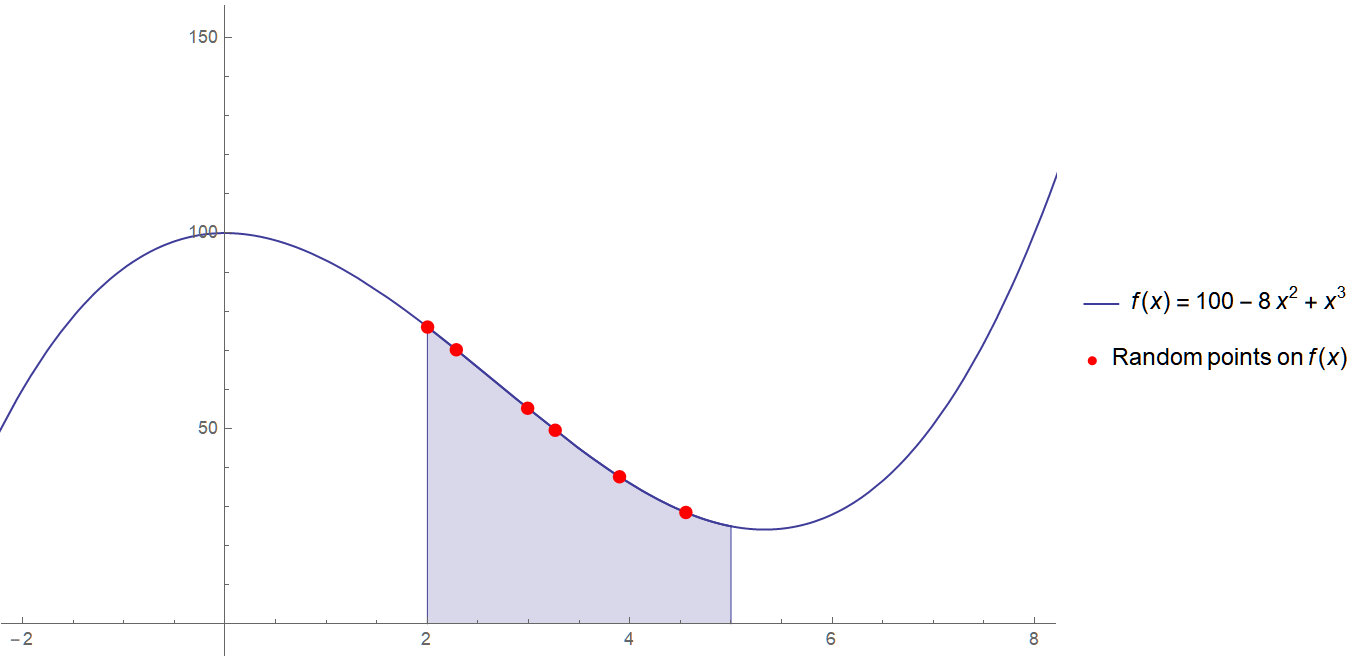
\includegraphics[width=10cm]{Images/pointsexample.png}
    \caption{The plot of f(x) and 6 random points plotted on it.}
    \label{fig:pointsexample}
\end{figure}
\begin{figure}[!htb]
    \centering
    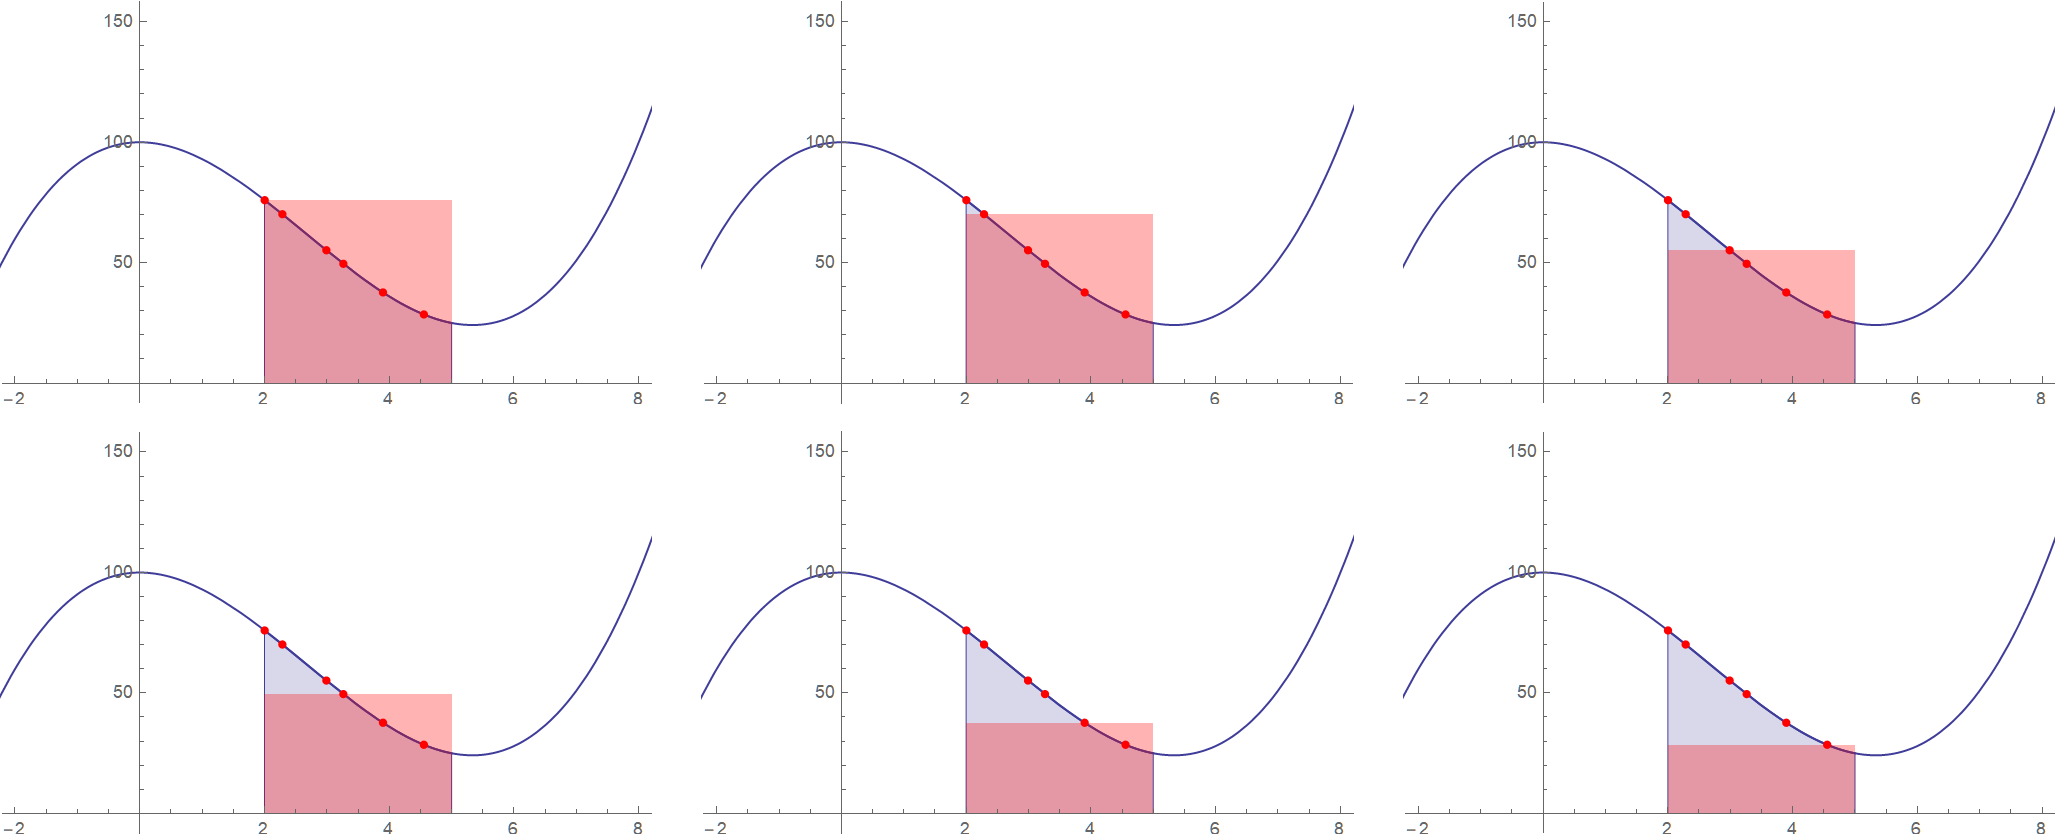
\includegraphics[width=10cm]{Images/rectexample.png}
    \caption{Rectangles of width $(b-a)$ with height corresponding to the random points.}
    \label{fig:rectexample}
\end{figure}\par
Recall eq. \ref{eq 2.3}, the multiplication of the $(b-a)$ term can be visualized as rectangles of width $(b-a)$ as above.
It is now clear to see that taking the mean of these rectangle areas will give us an approximation to the integral that improves with the addition of more points.
\clearpage
%----------------------------------------------------------------------------------------
%	Section 3
%----------------------------------------------------------------------------------------
\section{Estimating Pi}
In this section we will discuss the concepts of  the  Monte  Carlo  technique  for  estimating  the  value  of  pi( $\mathbf{\pi}$).

\subsection{Elementary Method}
In order to estimate the value of pi using Monte Carlo simulations we will estimate the area of a unit circle inscribed in a unit square.
\par
The  experiment is  conducted by taking random sample points in the region of the unit square. For  an unbiased estimator of area of the circle it is assumed  that the  random sample  points are uniformly distributed.
\par
The bounding box area is  $A_{box}=r^2=1$ and the area of the unit circle inscribed in the square is $A_{circle}=\pi r^2=\pi$. With $N_{box}$ total sample points and $N_{circle}$ is the total sample points lying inside the unit circle.
\par
Since the sample points are uniformly distributed within the bounding box, the ratio of the circle to the area of the  bounding  box is  approximately  equal  to  the ratio  of the number  of  sample  points  falling  in  the circle to the number of points falling in the bounding box.
\begin{align}
   \frac{A_{pi}}{A_{box}}=\frac{\pi r^2}{r^2}=\pi\approx \frac{N_{pi}}{N_{box}} 
\end{align}
\par An example of a single experiment is shown below.
\begin{figure}[!htb]
    \centering
    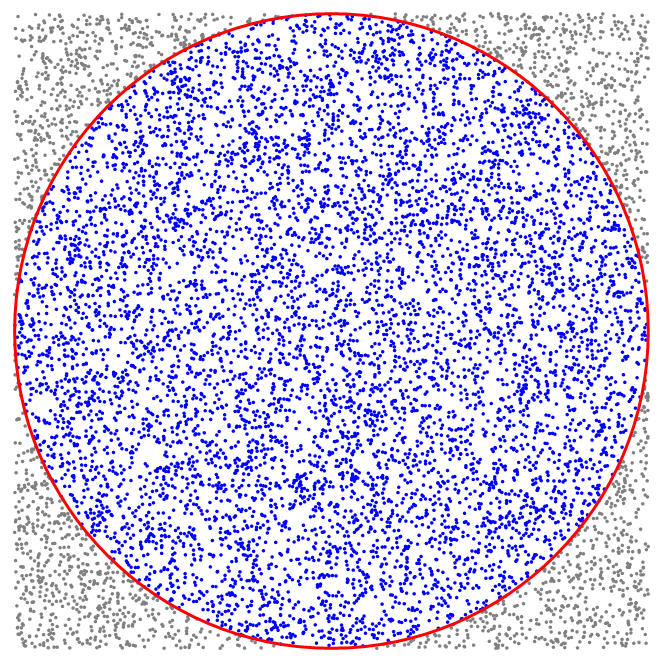
\includegraphics[width=8cm]{Images/piexample.png}
    \caption{Experiment with 10,000 points, $N_{pi}/N_{box}=3.1512$}
    \label{fig:piexample}
\end{figure}\par
We now repeat the experiment $10^3$ times with $10^6$ points. Taking the mean of these $10^3$ experiments gives us the following approximation. $\pi \approx 3.14154 \pm 0.00165$, with $ -1.696 \cdot 10^{-3}\ \%$ error.
\begin{figure}[!htb]
    \centering
    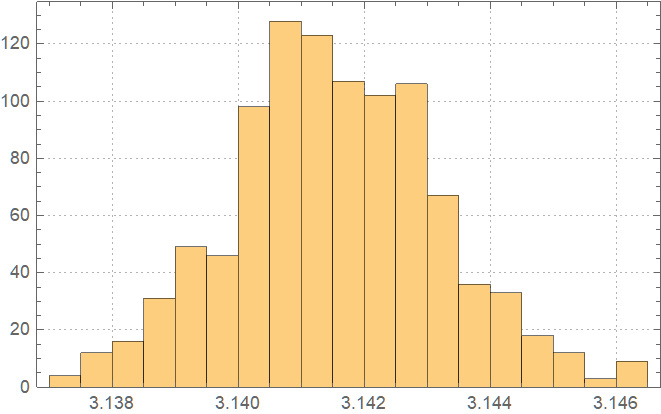
\includegraphics[width=10cm]{Images/repeatedpi.png}
    \caption{Histogram of experiment with $10^6$ points, repeated $10^3$ times.}
    \label{fig:repeatedpi}
\end{figure}

\subsection{Buffon's Needle}
 \textit{“A large plane area is ruled with equidistant parallel lines, the distance between two consecutive lines
of the series being a. A thin needle of length $l< a$ is tossed randomly onto the plane. What is the probability that the needle will intersect one of the lines?"}\par
 This forms the basis of the Buffon’s Needle problem. Which can be solved using elementary integral calculus \cite{needlewang}. Based on this analytical solution, the experiment can be used to approximate $\pi$ using Monte Carlo simulations.
\begin{theorem}
The probability of a needle intersecting a line is given by $p=\frac{2l}{a \pi}$.
\end{theorem}
 For a given needle of length "l" we model the dropping of the needle on the ruled plane with parallel lines "a" units apart as follows. \par
 Let x be the distance from the center of the needle to the nearest line and $\theta$ be the acute angle between the needle and the lines. Let x be a uniform random variable over the interval
\par
The uniform probability density function of x between 0 and $ \frac{t}{2}$ is
\[
\begin{cases}
   \dfrac{2}{a} & 0 \leqslant x\leqslant \dfrac{a}{2}\\
  0 & \text {   otherwise}
\end{cases}
\]
\par
and $\theta$ a uniform random variable over the interval $\left(0, \frac{\pi}{2}\right)$ with the probability density function:\\
\[
\begin{cases}
    \dfrac{2}{\pi} & 0 \leqslant x\leqslant \dfrac{\pi}{2}\\
    0 & \text {   otherwise}
\end{cases}
\]
\par
The two random variables, $x$ and $\theta$, are independent  Therefore the joint probability density function of
$(x,\theta)$ 
\[
\begin{cases}
    \dfrac{4}{a\pi} &  0 \leqslant x\leqslant \dfrac{a}{2} \text{ and } 0 \leqslant x\leqslant \dfrac{\pi}{2}\\
0  &  \text {   otherwise}
\end{cases}\]
\par
 for the short needle case $\left( l \leqslant a \right)$  A needle
intersects a line if
\begin{align*}
    \left( x \leqslant \frac{l}{2}\sin \theta \right )
\end{align*}
\par
The probability that the needle will intersect a line is

\begin{align*}
p=\int_{0}^\frac{\pi}{2}\int_{0}^{\frac{l}{2} \sin \theta} f(x,\theta)\ dx\ d\theta = \int_{0}^\frac{\pi}{2}\int_{0}^{\frac{l}{2} \sin \theta} \frac{4}{a\pi}\ dx\ d\theta = \frac{2l}{a\pi} 
\end{align*}

\begin{align*}
    p =\frac{2l}{a\pi} \QED
\end{align*}
\par
The p value can be estimated through Buffon's needle experiment. If the experiment contains n needles and there are m needles intersect lines, then the probability p can be estimated by the proportion
\begin{align}
    \widehat{p}&=\frac{m}{n} \nonumber
    \intertext{$\pi$ can therefore be estimated by}
    \widehat{\pi}&=\frac{2nl}{ma}
\end{align}\par
An example of a single experiment with 1000 needles is shown below.
We then repeat the experiment $10^3$ times with $10^6$ needles. Taking the mean of these $10^3$ experiments gives us the following approximation. $\pi \approx 3.14018 \pm 0.04510$, with $ -4.481 \cdot 10^{-2}\ \%$ error.
\begin{figure}[!htb]
    \centering
    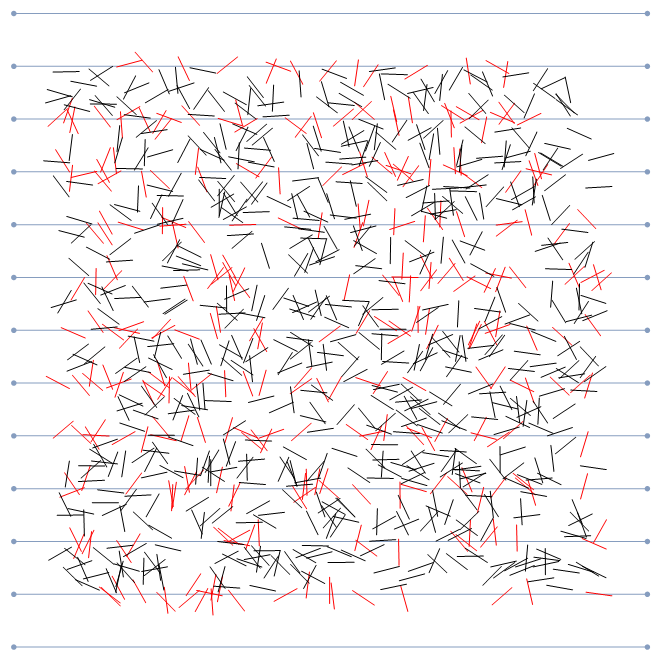
\includegraphics[width=10cm]{Images/needleexample.png}
    \caption{Experiment with 1000 needles, $\widehat{\pi}=3.14465$}
    \label{fig:needleexample}
\end{figure}\par

\begin{figure}[!htb]
    \centering
    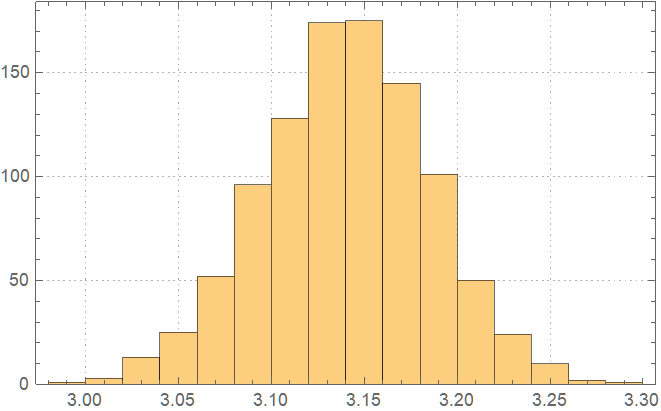
\includegraphics[width=10cm]{Images/repeatedneedle.png}
    \caption{Histogram of Buffon's needle experiment with $10^4$ needles, repeated $10^3$ times.}
    \label{fig:repeatedneedle}
\end{figure}

\clearpage
\subsection{Buffon's Noodle}
In this case we will estimate $\pi$ using Buffon's noodle problem. Buffon's noodle poses the question, "What is the expected number of crossings if we don't drop rigid needles but rather a flexible noodle?". \par       
For  straight needle N  there are exactly n line crossing for exactly n intersection of needles with the infinite grid giving us the expectation of line crossing as $E(N)=\frac{2a}{\pi d}$. where a is the length of needle. using the corollary of this result 
 that E(N) is a function of the length of the needle
only, not its shape \cite{noodle}.
\begin{theorem}
Let N be a noodle of length 't' thrown at random onto an infinite
grid of parallel lines with common distance d between them. Then the expected number of line-crossings E(N) is given by E(N) = $\frac{2t}{\pi d}$. 
\end{theorem}
\par
We remark that our definition of line-crossing demands that we count as  distinct crossings in the event that the noodle crosses the same line in different  places
In general if a needle intersects n times in m attempts, then a combination of “a”   such needles is expected to be intersected  “na” times in m attempts
If this combination is formed by infinitesimally  small needles , then it will become noodle\par
Lets choose a  sequence of polygonal lines $L_1$  $L_2$,$\cdots$ that approaches the curve N uniformly. The segments of the line $L_i$ we shall denote as $L_i1$, $L_i2$, · · · , $L_in$ and we
shall write $L_i=L_i1+L_i2+ \cdots +L_in $ 
letting $a_ij$ be the length of $L_{ij}$ such that $a_{ij}<d$ for all i and j 
 so that e($L_ij$) is
just the probability that $L_ij$ crosses a line,
 e($L_ij$) =$ 2a/\pi d$ Now letting $a_i$
be the length of $L_i$, we know that $a_i$ approaches a as i tends to infinity. Hence,
if $e(L_i) = e(L_j) + \cdots +e(L_n) $for all i, then 
\begin{equation}
    e(L_i) = \sum (2a_i/ \pi d) = (2/\pi d) \sum (a_ij) = (2/\pi d)a_i
\end{equation}
hence in the limit 
\begin{align}
e(N)= \frac{2a}{\pi d}
\end{align}


\subsubsection{A note on the simulation of noodles}
Simulating a "noodle" isn't very straightforward computationally, since "noodles" aren't very well defined. We choose to simulate it by considering a line of length $l$ divided into a random number of segments (between 5 and 10), and then randomizing the angles between the segments. One could also choose the make smooth noodles, by using bezier curves instead.
\par 
An example of a single experiment with 1000 noodles is shown  below.\
We now repeat the experiment $250$ times with $10^4$ noodles. Taking the mean of these $250$ experiments gives us the following approximation. $\pi \approx 3.18615 \pm 0.04602$, with $ + 1.418\ \%$ error.
\begin{figure}[!htb]
    \centering
    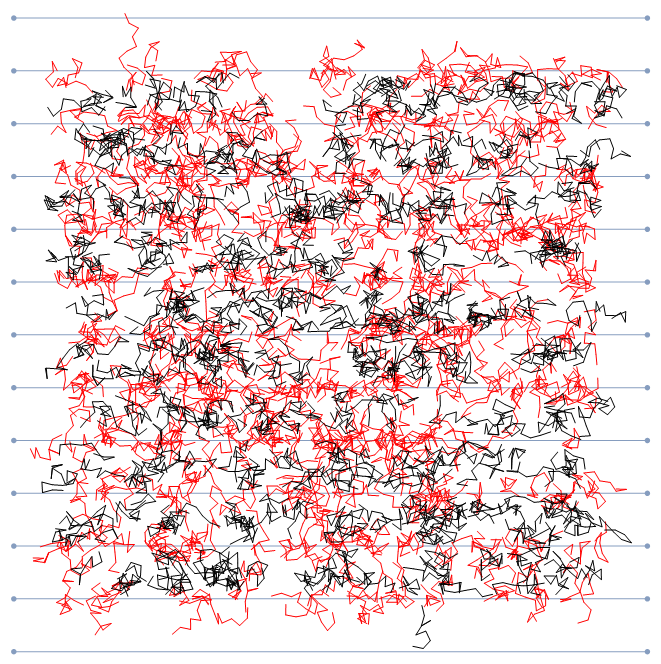
\includegraphics[width=10cm]{Images/noodleexample.png}
    \caption{Experiment with 1000 noodles, $\widehat{\pi}=3.36984$}
    \label{fig:noodleexample}
\end{figure}\par

\begin{figure}[!htb]
    \centering
    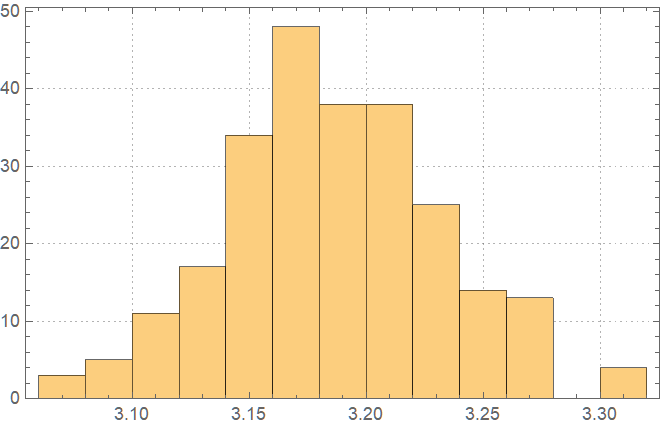
\includegraphics[width=10cm]{Images/repeatednoodle.png}
    \caption{Histogram of Buffon's noodle experiment with $10^4$ needles, repeated $250$ times.}
    \label{fig:repeatednoodle}
\end{figure}
\clearpage
%----------------------------------------------------------------------------------------
%	Section 4
%----------------------------------------------------------------------------------------
\section{Estimating Euler's number}
If $U_1, U_2 \cdots U_n$ are some independent and uniformly distributed random variables over (0,1). Let $S_n=\sum_{i=1}^n U_i$ and if $N$ is the minimum value of $n$ for which $S_n>1$. The expectation of N is in fact equal to $e$.
\par This problem originated from as a exercise from a famous Russian textbook by Gnedenko \cite{gnedenko}. For this section we will be drawing from two papers written by K. G. Russel on this topic \cite{simplerussell, russell_1983}.
\begin{theorem}
For iid uniform r.v. $U_1, U_2 \cdots U_n$ over (0,1), with $S_n=\sum_{i=1}^n U_i$ and if $N$ is the minimum value of $n$ for which $S_n>1$, then $E[N]=e$.
\end{theorem}
    Note that our goal is to show that 
\begin{align}   
    E[N]=\sum_{n=2}^{\infty}n P(N=n) = e
\end{align}
% Attempt 1
% If we can show that $P(N=n)=\frac{n-1}{n!}$, then we are done. Hence we continue as follows,
% \begin{align*}
%     P(N=n)&=P(S_{n}>1 \wedge S_{n-1}<1)\\
%     &=P(S_n>1)P(S_{n-1}<1)=P(S_{n-1}<1)-P(S_{n}<1)
% \end{align*}
% We have further simplified our problem, now all that remains is to find $P(S_n<1).$ We shall prove that $P(S_n<1)=1/n!$ using induction.\\
% Base case n=1,
% \begin{align*}
%     P(S_1 < 1) &= 1 = \frac{1}{1!}
%     \intertext{Assume it holds true for n, consider n+1}
%     P(S_{n+1} < 1) &= P(S_{n}<1) P(U_{n+1}<1-S_n)
%     \intertext{Assume $S_n=m$ for some $m \in (0, 1)$????}
%     &=P(S_n<1) P(U_{n+1}<1-m)\\
%     &=P(S_n<1) (1-m)\\
%     \intertext{If $m=n/(n+1)$ then we are done}
% \end{align*}
% % Attempt 2 
% If we can show that $P(N=n)=\frac{n-1}{n!}$, then we are done. Hence we continue as follows,
% \begin{align*}
%     P(N=n)&=P(S_{n}>1 \wedge S_{n-1}<1)\\
%     &=P(S_n>1)P(S_{n-1}<1)=P(S_{n-1}<1)-P(S_{n}<1)
% \end{align*}
% We have further simplified our problem, now all that remains is to find $P(S_n<1).$ We shall prove that $P(S_n<1)=1/n!$ using induction.\\
% Base case n=1,
% \begin{align*}
%     P(S_1 < 1) &= 1 = \frac{1}{1!}
%     \intertext{Assume it holds true for n.}
%     \intertext{Denote $P(S_n<1)$ as $F_{n}(1)$ and $P(x<1)$ for some $U_i$ as $F(1)$. Consider now the convolution of these two functions. We have to prove the following,}
%     F_{n} \textasteriskcentered F &= \frac{1}{(n+1)!}\\
%     F_{n} \textasteriskcentered F &= \frac{d}{ds}\left. \left( \int_{\mathbb{R}}F_{n, 1}(x, s-x) \right) \right|_{s=1}
% \end{align*}
If we can show that $P(N=n)=\frac{n-1}{n!}$, then we are done. Hence we continue as follows,
\begin{align*}
    P(N=n)&=P(S_{n}>1 \cap S_{n-1}<1)\\
    &=P(S_n>1)P(S_{n-1}<1)=P(S_{n-1}<1)-P(S_{n}<1)
\end{align*}
We have further simplified our problem, now all that remains is to show that $P(S_n<1)=\frac{1}{n!}$. This would complete the proof. We use the CDF of the Irwin-Hall distribution \cite{hall}.
\par The Irwin-Hall distribution is simply defined as, the sum of n independent and identically distributed, uniform distributions defined on the unit interval. The CDF of Irwin-Hall distribution is given as \footnote{This can be derived by integrating the pdf, which is in turn derived by induction by taking the convolution of $f_n \ast f$ to prove the $n+1^{th}$ case.}, 
\begin{align*}
    F(x)&=\frac{1}{n!} \sum_{k=0}^{\lfloor x \rfloor} (-1)^k \binom{n}{k} (x-k)^n
    \intertext{For x=1}
    F(1)&=P(S_n<1)=\frac{1}{n!} \sum_{k=0}^{1} (-1)^k \binom{n}{k} (1-k)^n=\frac{1}{n!} \QED 
\end{align*}
\par The astute reader may ask what is $E[N]$ if we consider $S_n>a$ for any real number $a$? This general form is answered in the paper by Russell \cite{russell_1983}.
\par We now continue with the simulation to predict $e$ by choosing $10^6$ random uniform numbers between (0,1) and counting the average number of times it takes for the sum to cross 1.
\par We now repeat the experiment $10^4$ times with $10^6$ numbers per experiment. Taking the mean of these $10^4$ experiments gives us the following approximation. $e \approx 2.71827 \pm 0.00087$, with $ - 3.405 \cdot 10^{-4}\ \%$ error.
\begin{figure}[!htb]
    \centering
    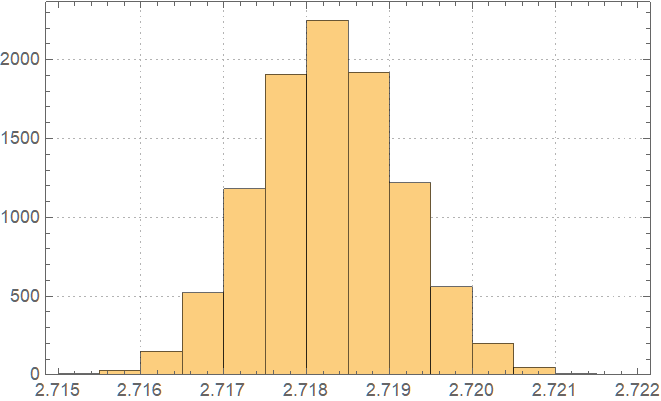
\includegraphics[width=10cm]{Images/repeatede.png}
    \caption{Histogram of $e$ experiment with $10^6$ numbers, repeated $10^4$ times.}
    \label{fig:repeatede}
\end{figure}
%----------------------------------------------------------------------------------------
%	Section 5
%----------------------------------------------------------------------------------------
\section{Estimating Euler-Mascheroni constant and Stieltjes constants}
We begin this section by defining the Euler-Mascheroni constant and Stieltjes constants.
\par The Euler Mascheroni Constant ($\gamma$) is defined as the limiting difference between the harmonic series and the natural logarithm, i.e.
\begin{align}
    \gamma &= \lim_{n \rightarrow \infty} \left( H_n - \log n \right)\\ \label{emconstant}
    &= \lim_{n \rightarrow \infty} \left(\sum_{k=1}^{n} \frac{1}{k} - \log n \right) \nonumber
\end{align}
\par Stieltjes constants can be thought of as a generalization of the Euler-Mascheroni constant, defined as,
\begin{align}
    \gamma_n &= \lim_{m \rightarrow \infty} \left( \sum_{k=1}^m \frac{(\log k)^n}{k} - \frac{(\log m)^{n+1})}{n+1} \right)
\end{align}
\par It is clear to see that $\gamma_0=\gamma$. It is interesting to note that Stieltjes constants were originally discovered in the Laurent series expansion (about 1) of the Riemann Zeta function \cite{stieltjeswolfram}.
\begin{align*}
    \zeta (z) = \frac{1}{z-1} + \sum_{n=0}^\infty \frac{(-1)^n }{n!} \gamma_n (z-1)^n
\end{align*}
We can in fact further generalize Stieltjes constants by considering the Laurent series of the Hurwitz-Zeta function instead of Riemann zeta. However, we will not further examine this.
\subsection{Euler-Mascheroni constant}
% We will first approximate $\gamma$ by using an integral representations of $\gamma$.\par
% We proceed by using the following two known integral representations of $H_n$ and $\log(n)$ in eq \ref{emconstant}.
% \begin{align*}
%     H_n &= \int_0^1 \frac{1-x^n}{1-x}\ dx\\
%     \log n &= \int_0^1 \frac{x^{n-1}-1}{\log x}\ dx
% \end{align*}
% \begin{theorem}
% $\gamma = \int_0^1 \frac{1}{1-x} + \frac{1}{\log x}\ dx$ 
% \end{theorem}
% \begin{align*}
%     \gamma &= \lim_{n \rightarrow \infty} (H_n - \log n)\\
%     &= \lim_{n \rightarrow \infty} \int_0^1 \left( \frac{1-x^n}{1-x} - \frac{x^{n-1}-1}{\log x}\ dx \right)
%     \intertext{Since the function inside the integral is uniformly convergent and bounded, by the Bounded Convergence Theorem we have,}
%     &= \int_0^1 \lim_{n \rightarrow \infty} \left( \frac{1-x^n}{1-x} - \frac{x^{n-1}-1}{\log x} \right)\ dx\\
%     &= \int_0^1 \frac{1}{1-x}+\frac{1}{\log x}\ dx
% \end{align*}
We will estimate the Euler-Mascheroni constant by first approximating the Gumbel distribution \cite{gumbelwolfram}.\par
The Gumbel distribution accepts two parameters, $\alpha$ and $\beta$. It is defined by the following probability density function,
\begin{align*}
    P(x)&=\frac{1}{\beta} e^{\frac{x-\alpha}{\beta}-e^{\frac{x-\alpha}{\beta}}}\\
    &= \frac{1}{\beta}\exp \left(\frac{x-\alpha}{\beta} - \exp \left( \frac{x-\alpha}{\beta} \right) \right)
    \intertext{and the following cumulative distributive function,}
    F(x)&=1-\exp \left( -\exp \left( \frac{x-\alpha}{\beta}\right) \right)
\end{align*}
It can be seen using integral representation of $\gamma$ that the mean of the Gumbel distribution is,
$$
    \mu = \alpha - \gamma \beta
$$
\par Our goal is therefore to simulate a Gumbel distribution with parameters $\alpha = 0$ and $\beta = -1$. The mean of this would therefore be $\gamma$.\par
We simulate the Gumbel distribution by using its quantile function (i.e. inverse CDF).
\par Calculating the inverse function for F(x) with $\alpha=0, \gamma=-1$ we get.
\begin{align}
   Q(p)&= \log \left(- \log \left(p\right)\right)
\end{align}
\par Where $p$ takes values between 0 and 1. Taking $n$ random points $p$ between 0 and 1, and taking the mean of their respective $Q(p)$ we approximate $\gamma$.
\par Taking $10^6$ points and repeating the experiment $10^4$ times gives us the following approximation $\gamma \approx 0.57721 \pm 0.00128$. With $-4.824 \cdot 10^{-4} \%$ error.
\begin{figure}[!htb]
    \centering
    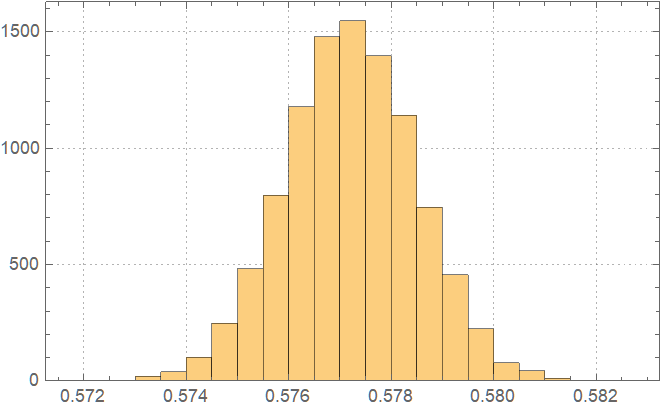
\includegraphics[width=10cm]{Images/repeatedgamma.png}
    \caption{Histogram of experiment with $10^6$ points, repeated $10^4$ times.}
    \label{fig:repeatedgamma}
\end{figure}
\subsection{Stieltjes constants}
Calculating Stieltjes constants is not a trivial task, there exist many infinite series representations of Stieltjes constants which converge very slowly \cite{stieltjeswolfram} (see eq.12). Extensive work has also been done in implementing fast algorithms to compute Stieltjes constants with high accuracy \cite{johansson2018computing}.
\par We will approximate a few Stieltjes constants by estimating the following integral definition.
\begin{align}
    \gamma_n = \frac{(-1)^n n!}{2 \pi} \int_0^{2 \pi} e^{nix} \zeta (e^{ix}+1)\, dx \label{5.4}
\end{align}
\par The above integral is derived by using Cauchy's differentiation formula on $$(-1)^n \gamma_n= \frac{d^n}{dz^n} \left. \left ( \zeta(z) - \frac{1}{z-1}\right)\right|_{z=1}$$
which is in turn derived by comparing the Laurent series of the Zeta function with a traditional Taylor series.
\par The reader should note that calculating Stieltjes constants with Monte Carlo integration is not at all practical due to the low accuracy. For practical approximations other forms of numerical integration techniques are used \cite{johansson2018computing, newtoncotes}.
\par We will estimate eq. \ref{5.4} using the crude Monte Carlo integration described in the first section. The following table shows the results we achieved.

\begin{table}[!htb]
\centering
\resizebox{\textwidth}{!}{%
\begin{tabular}{@{}cccccc@{}}
\toprule
$\gamma_n$ & \begin{tabular}[c]{@{}c@{}}No. of \\ points chosen\end{tabular} & \begin{tabular}[c]{@{}c@{}}No. of times \\ repeated\end{tabular} & \begin{tabular}[c]{@{}c@{}}Mean and\\ Standard Deviation\end{tabular} & Real values & Percentage Error \\ \midrule
$1$ & $10^5$ & $10^4$ & $-0.0728663 \pm 0.00258$ & $-0.0728159$ & $-2.00069 \cdot 10^{-2}$ \\
$2$ & $10^5$ & $10^4$ & $-0.00969426 \pm 0.00524$ & \multicolumn{1}{l}{$-0.0096904$} & $+4.02199 \cdot 10^{-2}$ \\
$3$ & $10^5$ & $1.5 \cdot 10^4$ & $+0.00204329 \pm 0.01551$ & $+0.0020538$ & $-5.13216 \cdot 10^{-1}$ \\
$4$ & $10^5$ & $3 \cdot 10^4$ & $+0.00233049 \pm 0.06136$ & \multicolumn{1}{l}{$+0.0023253$} & $+2.20283 \cdot 10^{-1}$ \\ \bottomrule
\end{tabular}%
}
\caption{Computed values of the first 4 Stieltjes constants (not including 0)}
\label{tab:stieltjescal}
\end{table}
\begin{figure}[!htb]
    \centering
    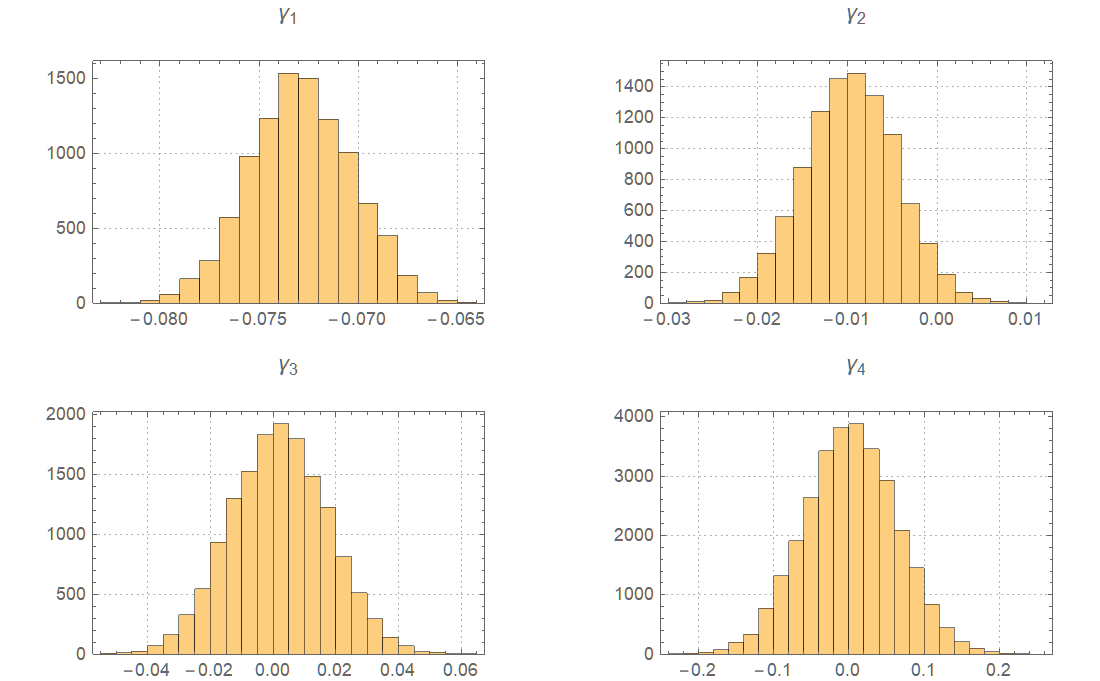
\includegraphics[width=\textwidth]{Images/stieltjesconstantsgrid.png}
    \caption{Histogram of the 4 experiments.}
    \label{fig:repeatedstieltjes}
\end{figure}
\clearpage
% --------------------------------------------------------------------------------
%	Section 6
%----------------------------------------------------------------------------------------
\section{Estimating Phi}
We conclude the estimation of mathematical constants on a lighter note.
\par Since $\varphi$ is an algebraic number, estimating $\varphi$ is very trivial. Since we know that $\varphi = \frac{1+\sqrt{5}}{2}$, we can simply choose an integral which evaluates to the desired result. We will choose $\int_4^5 \frac{3}{2}+\frac{1}{4 \sqrt{x}}\ dx$ which is evidently equal to $\varphi$.
\par We estimate the integral with the method described in Section 1.
\par We repeat the experiment $10^4$ times with $10^6$ points per experiment. Taking the mean of these $10^4$ experiments gives us the following approximation, $\varphi \approx 1.61803 \pm 3.79948 \cdot 10^-6$, with $6.544 \cdot 10^{-7}\ \%$ error. In fact the approximation is correct up to 7 decimal places.
\begin{figure}[!htb]
    \centering
    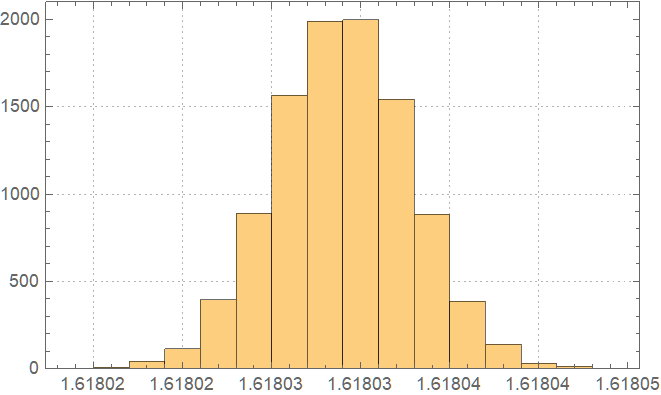
\includegraphics[width=10cm]{Images/repeatedphi.png}
    \caption{Histogram of experiment with $10^6$ points, repeated $10^4$ times.}
    \label{fig:repeatedphi}
\end{figure}
%----------------------------------------------------------------------------------------
%	Section 7
%----------------------------------------------------------------------------------------
\section{Quasi-Monte Carlo integration}
Throughout the project so far we have only considered what is known as "naive" Monte Carlo integration. We will now justify its nomenclature by listing out 2 modified methods of Monte Carlo integration that are so designed to reduce variability.
\par
Quasi-Monte Carlo integration is simply, Monte Carlo integration using quasi-random generated numbers to form the integration nodes (as opposed to pseudo-random in naive integration) \cite{MOROKOFF1995218}.
\subsection{Quasi-random sequences (low-discrepancy sequences)}
To make the above statement clearer, we will first define quasi-random numbers.
\par Quasi-random numbers are numbers generated from quasi-random sequences, which are in turn defined as sequences with low discrepancy \cite{quasirandomdiscrepancy}.


\section{Importance sampling}
\bibliographystyle{unsrt}
\bibliography{references}
\end{document}